\documentclass[
size=17pt,
paper=smartboard,
mode=present,
display=slidesnotes,
style=paintings,
nopagebreaks,
blackslide,
fleqn]{powerdot}

% styles: sailor, paintings
% wj capsules prettybox
% mode = handout or present


\usepackage{amsmath,graphicx,color,amsfonts}
\usepackage[brazilian]{babel}
\usepackage[utf8]{inputenc}
\newcommand{\palette}{Europa}


% palettes:
%    - sailor: Sea, River, Wine, Chocolate, Cocktail 
%    - paintings: Syndics, Skater, GoldenGate, Moitessier, PearlEarring, Lamentation, HolyWood, Europa, MayThird, Charon 

\newcommand{\cursopequeno}{EC01008 AOC}
\newcommand{\cursogrande}{\Large EC01008 -- Arquitetura e organização de computadores}



\author{Ronaldo de Freitas Zampolo\\FCT-ITEC-UFPA}
\date{2023-4}


\pdsetup{
   lf = {\cursopequeno},
   rf = {Memória interna}, palette = {\palette}, randomdots={false},
   cf = {\theslide}
}


%opening
\title{\cursogrande\\ \vspace{1cm}{Memória externa}}

\begin{document}
\maketitle[randomdots={false}]

\begin{slide}{Agenda}
      \tableofcontents[content=sections]
   \end{slide}

\section[slide=true]{Disco magnético}
\begin{slide}{Disco magnético}
	\begin{itemize}
		\item Substrato: superfície circular de material não magnético
		\item Materiais do substrato: 
			\begin{itemize}
				\item Alumínio
				\item Liga de alumíno
				\item Vidro (mais recentemente)
			\end{itemize}
		\item Benefícios do substrato de vidro:
			\begin{itemize}
				\item Aumento da confiabilidade do disco (superfície mais uniforme)
				\item Redução de erros nos processos de leitura e escrita
				\item Melhor rigidez (melhor dinâmica)
				\item Maior resistência a choques
			\end{itemize}
		\item O substrato é recoberto com um material magnetizável.
	\end{itemize}
\end{slide}

\begin{slide}{Mecanismos de escrita e leitura}
	\begin{itemize}
		\item Escrita:
			\begin{itemize}
				\item A direção da corrente elétrica, gera um campo magnético orientado
				\item O campo magnético determina a orientação da magnetização no disco
			\end{itemize}
		\item Leitura:
			\begin{itemize}
				\item Em discos mais antigos, é o mesmo cabeçote para escrita e leitura
				\item Em discos recentes, é usado um material magneto-resistente 
			\end{itemize}
	\end{itemize}
	\begin{figure}[h]
		\centering
		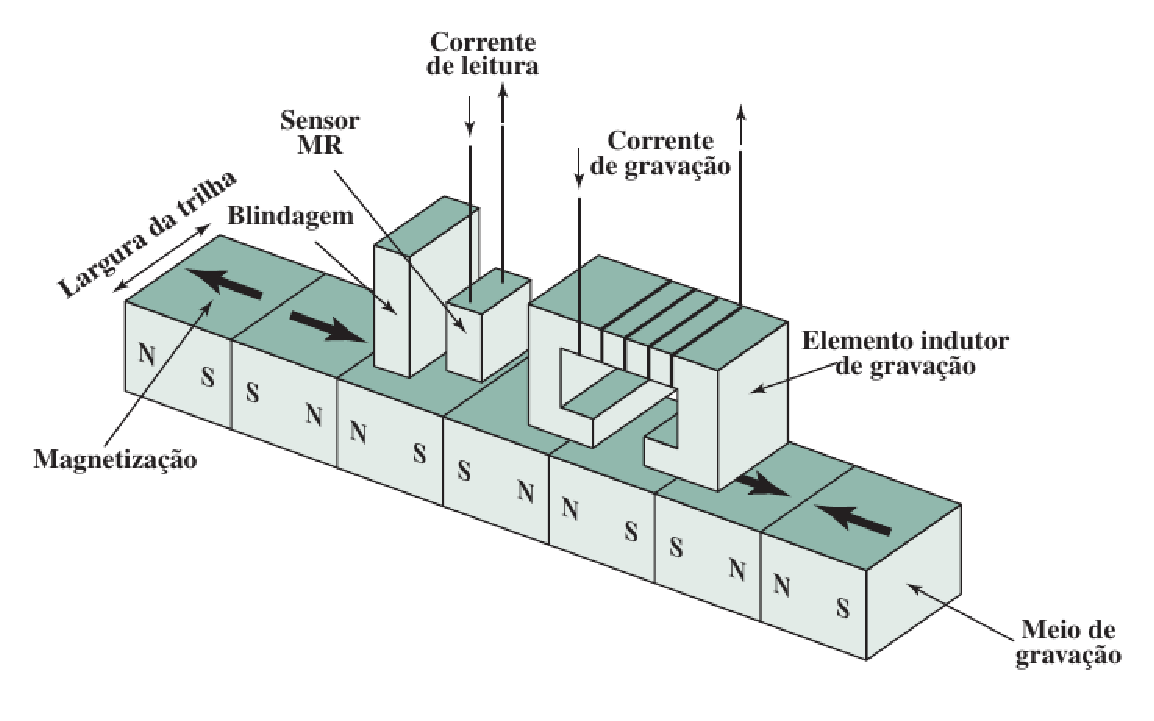
\includegraphics[width=0.45\textwidth]{figs/cabeca-gravacao-leitura}
	\end{figure}
\end{slide}

\begin{slide}{Organização dos dados}
	\begin{itemize}
	%	\item Organização dos dados:
	%		\begin{itemize}
				\item Trilhas: 
					\begin{itemize}
						\item Anéis concêntricos
						\item Mesma largura que os cabeçotes
						\item Há milhares por superfície
					\end{itemize}
				\item Intertrack gaps: 
					\begin{itemize} 
						\item Separação entre trilhas, com objetivo de redução de \emph{erros}
						\item \emph{Desalinhamento de cabeçote}
						\item \emph{Interferência de campos magnéticos}
					\end{itemize}
				\item Setores: 
					\begin{itemize}
						\item Unidades de transferência de dados
						\item Há centenas por trilha
						\item Tamanhos fixos ou variáveis (512 bytes é usado na maioria dos sistemas)
					\end{itemize}
				\item Intersector gaps: separação entre setores
	%		\end{itemize}
	\end{itemize}
\end{slide}

\begin{slide}{Organização dos dados}
	\begin{itemize}
		\item Organização dos dados (https://www.youtube.com/watch?v=NtPc0jI21i0)
			\begin{figure}[h]
				\centering
				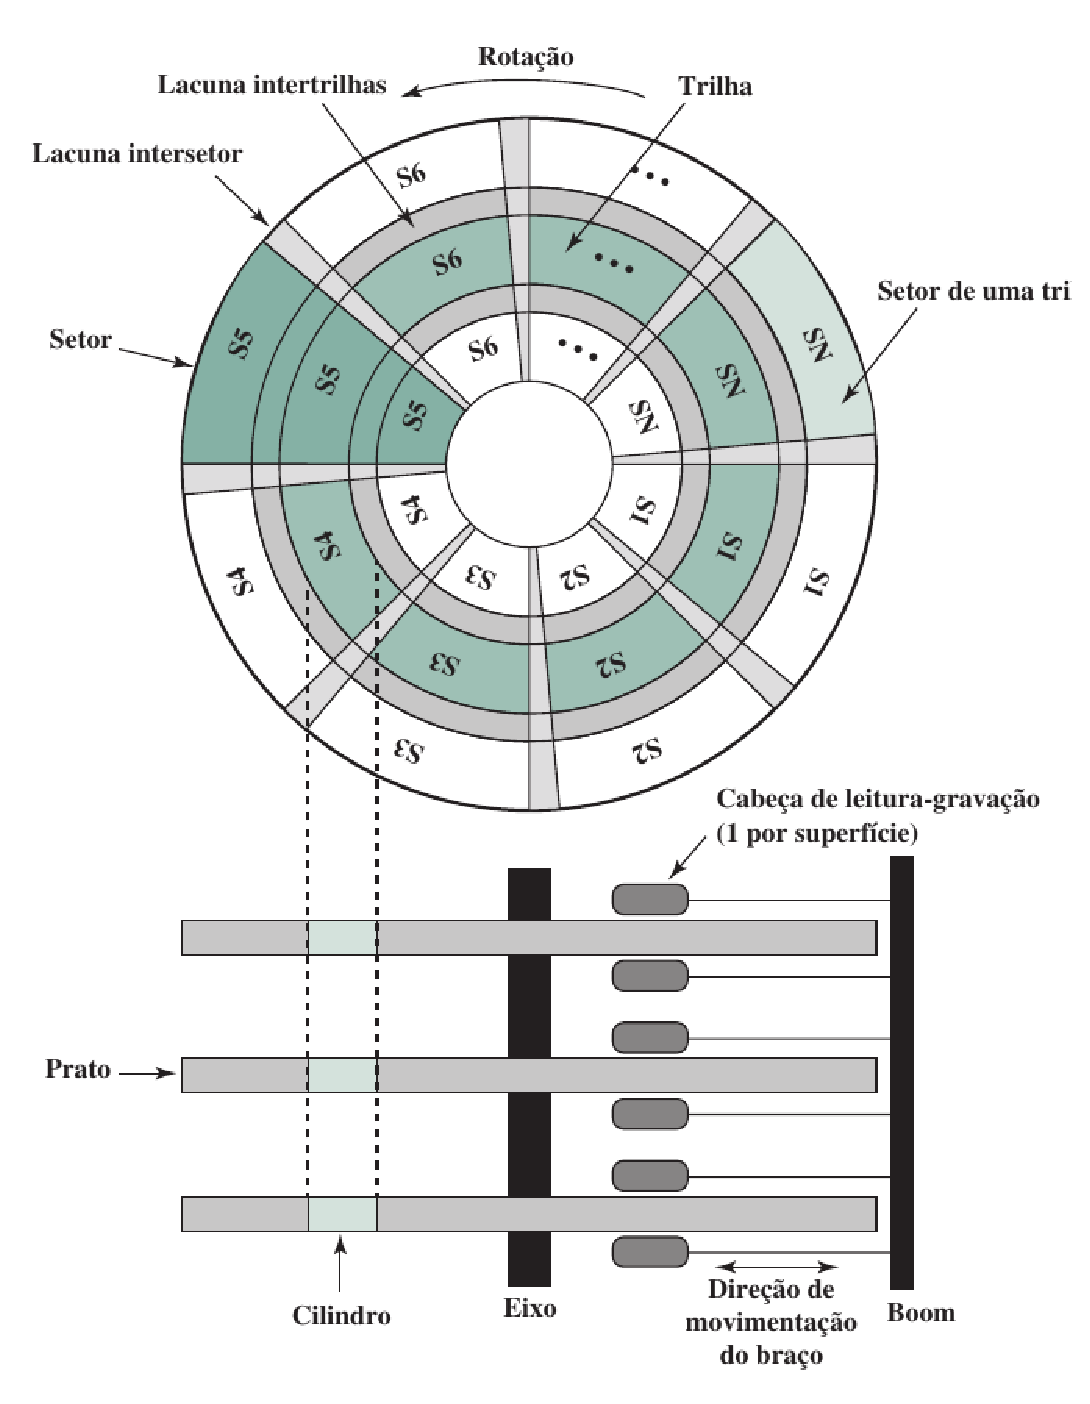
\includegraphics[width=0.38\textwidth]{figs/layout-disco}
				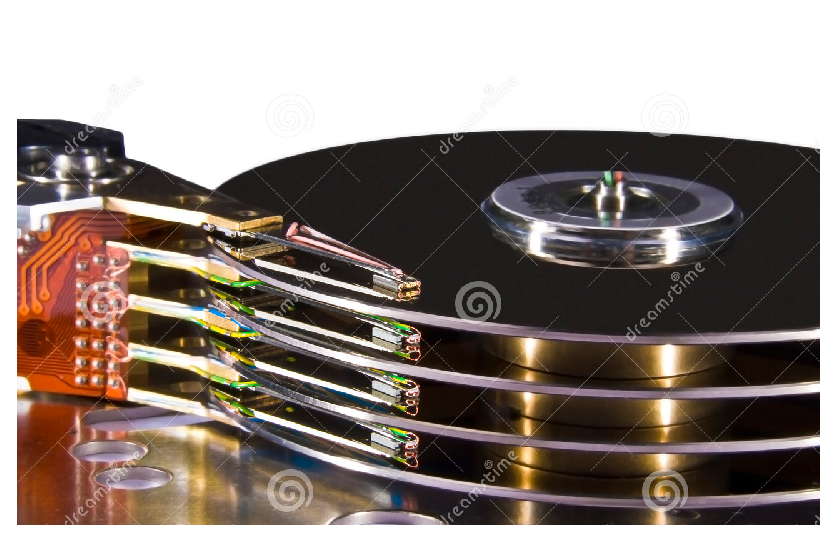
\includegraphics[width=0.55\textwidth]{figs/hd}
			\end{figure}
	\end{itemize}
\end{slide}

\begin{slide}{Organização dos dados}
	\begin{itemize}
		\item A velocidade linear varia com a distância em relação ao centro do disco
		\item Para garantir a mesma taxa de bits, o espaçamento entre estes diminui quanto mais externa for a trilha (velocidade angular constante - CAV)
			\begin{itemize}
				\item Vantagem: acesso a blocos de dados diretamente por trilha e setor
				\item Desvantagem: trilhas mais externas possuem menor densidade de bits
				\item Solução: densidade variável em cada trilha (resulta em circuitos mais complexos)
			\end{itemize}
		\item Gravação em múltiplas zonas (MZR):
			\begin{itemize}
				\item A superfície é dividida em zonas concêntricas (tipicamente 16)
				\item Cada zona contém um número de trilhas contíguas (milhares)
				\item Em cada zona, o número de bits por trilha é constante
				\item Zonas mais distantes do centro contém mais bits (mais setores)
				\item A densidade de bits é aproximadamente constante em toda a superfície do disco
			\end{itemize}
	\end{itemize}
\end{slide}

\begin{slide}{Organização dos dados}
	\begin{itemize}
		\item Comparação entre CAV e MZR
			\begin{figure}[h]
				\centering
				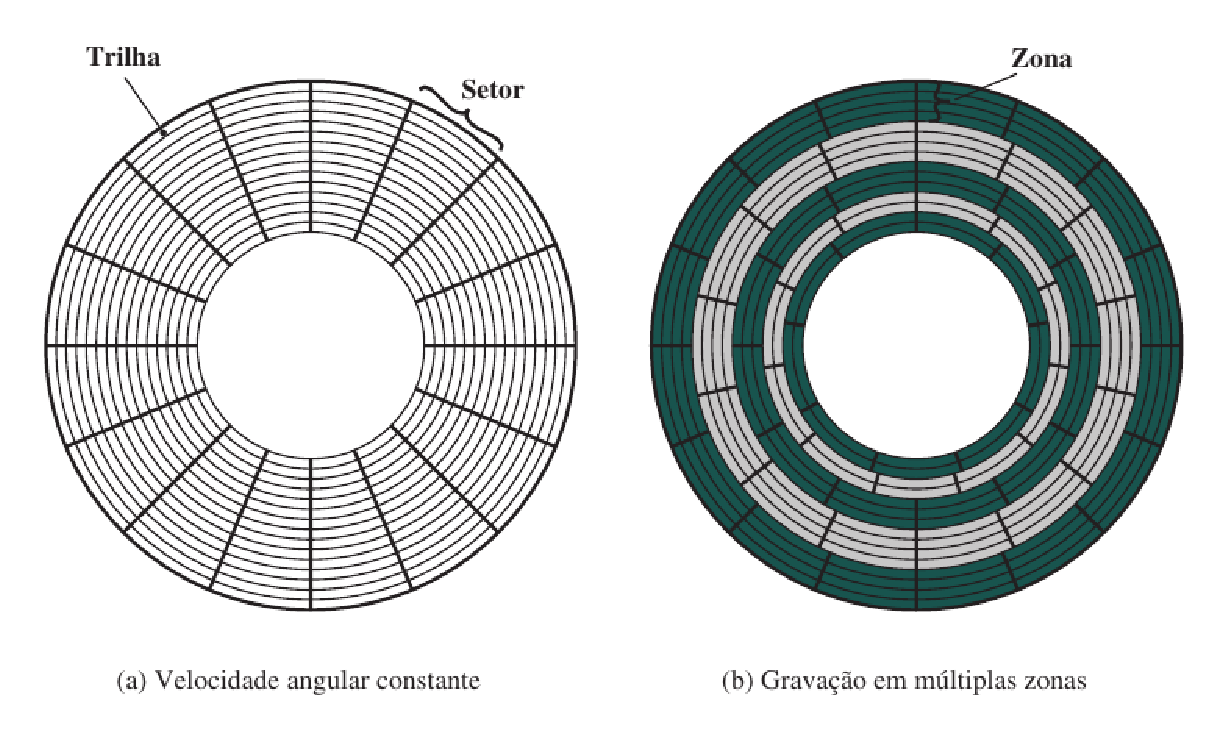
\includegraphics[width=0.8\textwidth]{figs/comparacao-layout}
			\end{figure}
	\end{itemize}
\end{slide}

\begin{slide}{Formatação}
	\begin{itemize}
		\item É necessário localizar/identificar cada setor em uma trilha
		\item Marcadores de início de trilha e de início e fim de setores
		\item Dados de formatação do disco (transparentes para o usuário)
		\item Exemplo:
			\begin{itemize}
				\item Cada trilha: 30 setores
				\item Cada setor: 600 bytes (total), 512 bytes (dados)
			\end{itemize}
	\end{itemize}
			\begin{figure}[h]
				\centering
				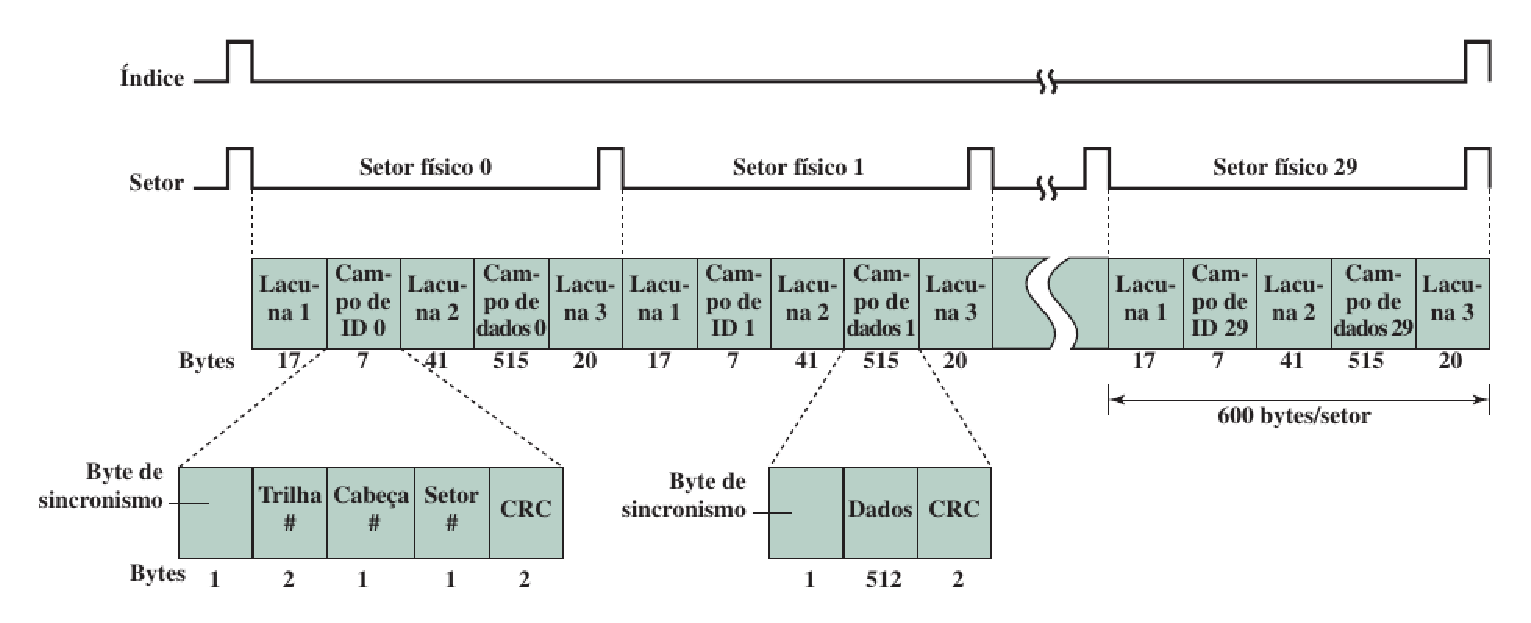
\includegraphics[width=0.7\textwidth]{figs/formato-winchester}
			\end{figure}
\end{slide}

\begin{slide}{Características físicas}
	\begin{itemize}
		\item Principais características físicas
			\begin{figure}[h]
				\centering
				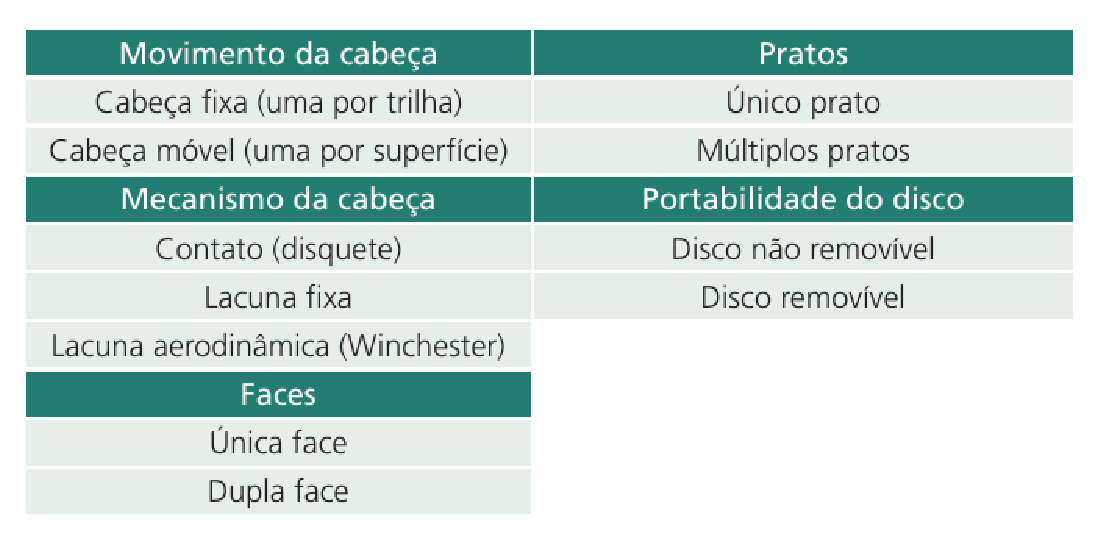
\includegraphics[width=0.7\textwidth]{figs/caracteristicas-fisicas-disco}
			\end{figure}
	\end{itemize}
\end{slide}

\begin{slide}{Parâmetros de desempenho}
	\begin{itemize}
		\item Tempo de busca (\emph{seek time}): tempo necessário para posicionamento da cabeça na trilha correta
		\item Latência (\emph{rotational latency}): tempo para alcançar o início do setor
		\item Tempo de acesso (\emph{access time}): tempo de busca + latência
		\item Tempo de transferência de dados (\emph{transfer time})
			\begin{figure}[h]
				\centering
				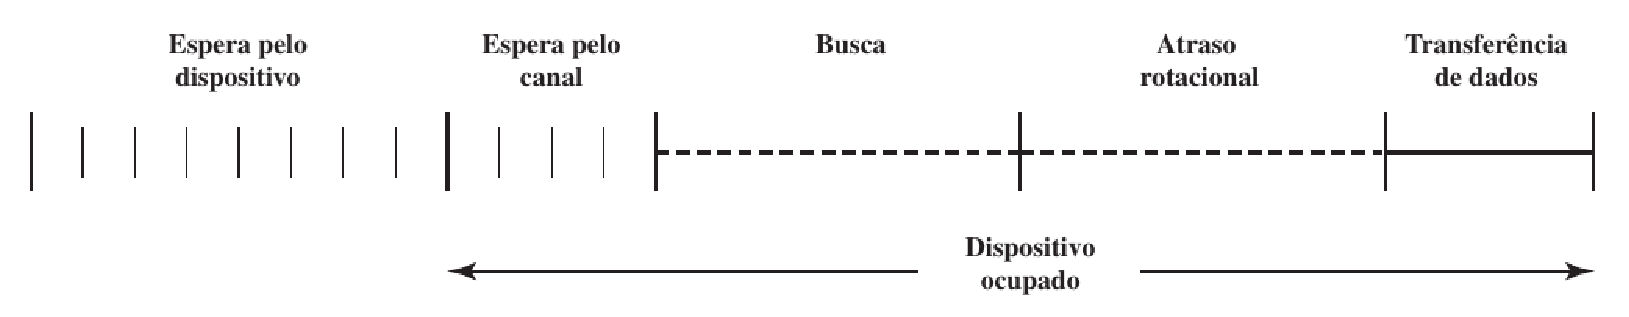
\includegraphics[width=0.8\textwidth]{figs/temporizacao}
			\end{figure}
		\item Tempo total
			\begin{equation*}
				T_\text{total} = T_\text{busca} + T_\text{latência} + T_\text{transferência} = T_\text{busca} + \frac{1}{2r} + \frac{b}{rN}
			\end{equation*}
			onde $r$, $b$, e $N$ representam a velocidade de rotação, o número de bytes a ser transferido, e o número de bytes em uma trilha, respectivamente.
	\end{itemize}
\end{slide}
\begin{slide}{Parâmetros de desempenho}
	\begin{itemize}
		\item Parâmetros típicos
			\begin{figure}[h]
				\centering
				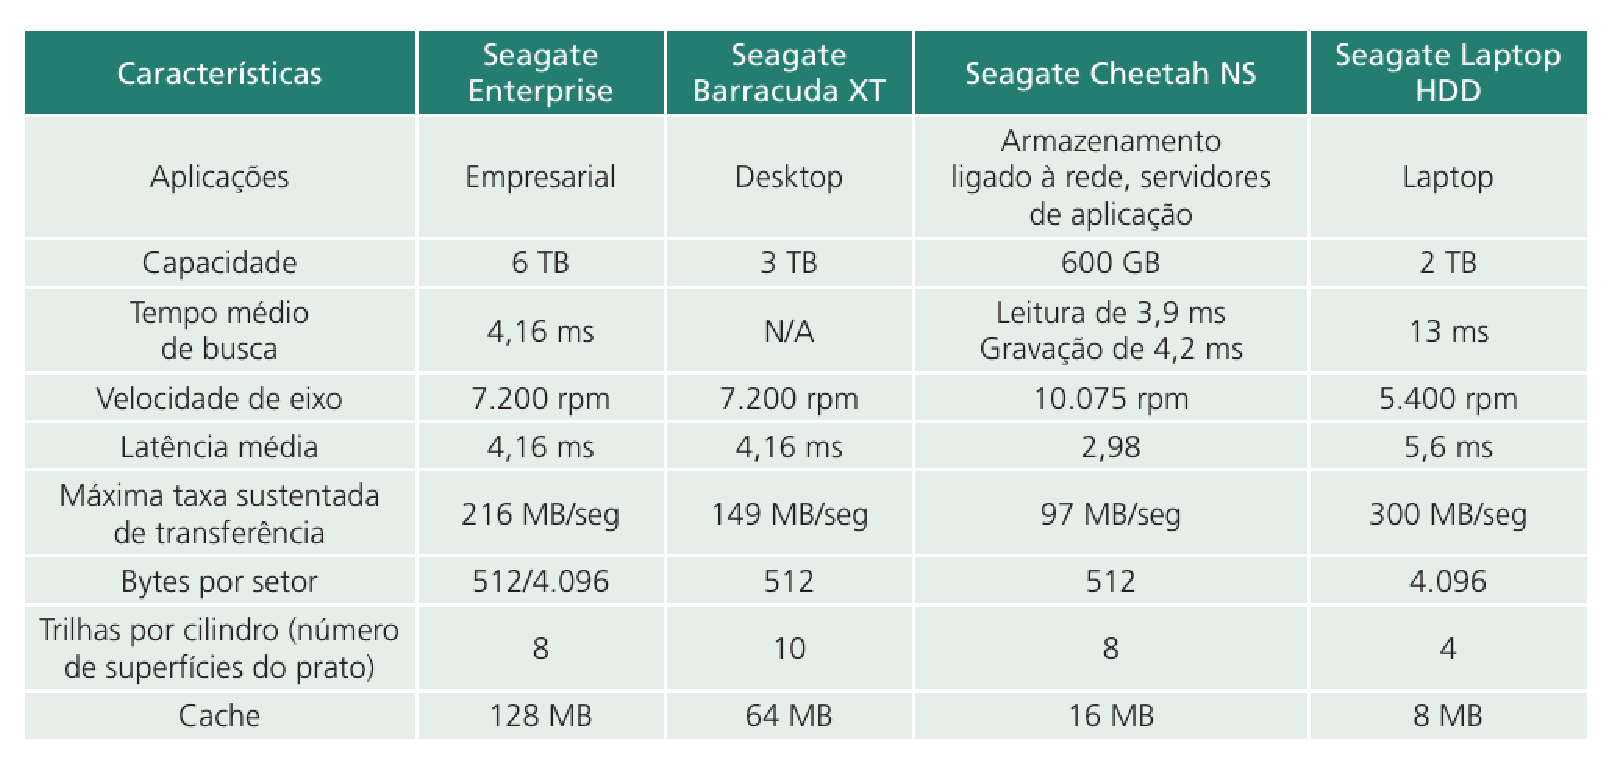
\includegraphics[width=0.9\textwidth]{figs/parametros-drive}
			\end{figure}
	\end{itemize}
\end{slide}

\section[slide=true]{RAID}
\section[slide=true]{Drives de estado sólido}
\section[slide=true]{Memória óptica}
\section[slide=true]{Fita magnética}
\section[slide=true]{Memória principal semicondutora}

% \section[slide=True]{Memória flash}
% \begin{slide}{Memória flash}
% \end{slide}
%
% \section[slide=True]{Novas tecnologias de memórias de estado sólido não-voláteis}
% \begin{slide}{STT-RAM}
% \end{slide}
%
% \begin{slide}{PCRAM}
% \end{slide}
%
% \begin{slide}{ReRAM}
% \end{slide}
%


\end{document}
